\documentclass[11pt]{article}
% Default margins are too wide.
\setlength{\topmargin}{-.5in}
\setlength{\textheight}{9in}
\setlength{\oddsidemargin}{.125in}
\setlength{\textwidth}{6.25in}

\usepackage{graphicx}
\usepackage{wrapfig}

\begin{document}
\title{CS 6316 - Homework 1 Report}
\author{Donnie Newell}
\date{February 18, 2013}
\maketitle


\section{Summary of Results}
Predicting spam e-mail is a relevant, practical topic for machine learning. Both tree-based methods and rule-based approaches were able to achieve classification accuracies above 88\%. In the end, the JRip rule based method offered the most attractive model, with high accuracy and low complexity.
\section{Problem Description}
Any user of e-mail understands the problem with "spamming" or mass unsolicited "cold-call" email. It can be for malicious purposes, such as identity theft, or less harmful activities such as marketing. The growth of spam e-mail has motivated the automated detection and filtering of it.

This analysis was conducted on 4,601 observations of spam and non-spam email. There are 57 fields that describe the presence of various word and character patterns in the e-mails. The last field describes whether or not the email was categorized as spam, or not. 

When analyzing the performance of tree and rule-based models, the main metrics of interest are related to classification accuracy and complexity of the model. For trees, complexity is represented in the number of nodes and leaves in the tree, while 

 Weka Explorer \cite{Halletal2009} was used to perform all of the analysis of the spam data. The pre-processing, classification, attribute selection and visualization functions were used in this assignment.
 
\section{Decision Trees}
\subsection{ID3}
In order to use ID3 on the spam data, the continuous frequencies had to be discretized. The attributes were divided into 10 bins using the supervised discretization filter in Weka. After running the ID3 algorithm, a classification accuracy of 81.18\% was achieved. The decision tree generated was very complex. 

To reduce the size of the tree, the CfsSubsetEval attribute selection filter was used. This filter provides a list of attributes that provide the most predictive ability for classification. When running the ID3 model on this subset of attributes, the classification accuracy went down to 80.24\%. Attribute selection reduced the number of attributes from 58 to 16, and the tree was much smaller, although still unwieldy.

The final attempt to improve the classification accuracy of ID3 was to use unsupervised discretization with findNumBins turned on. This means that the filter will try to find the optimal number of equal width bins to discretize each attribute into. The ID3 model trained on this data produced 88.7\% classification accuracy, up 7\% over the first discretization approach. See Figure \ref{fig:id3_remove_error} for classification error of the frequency of the word "remove" in this data set. As you can see, the predictive ability is fairly good.
\begin{figure}[here]
	\centering	
	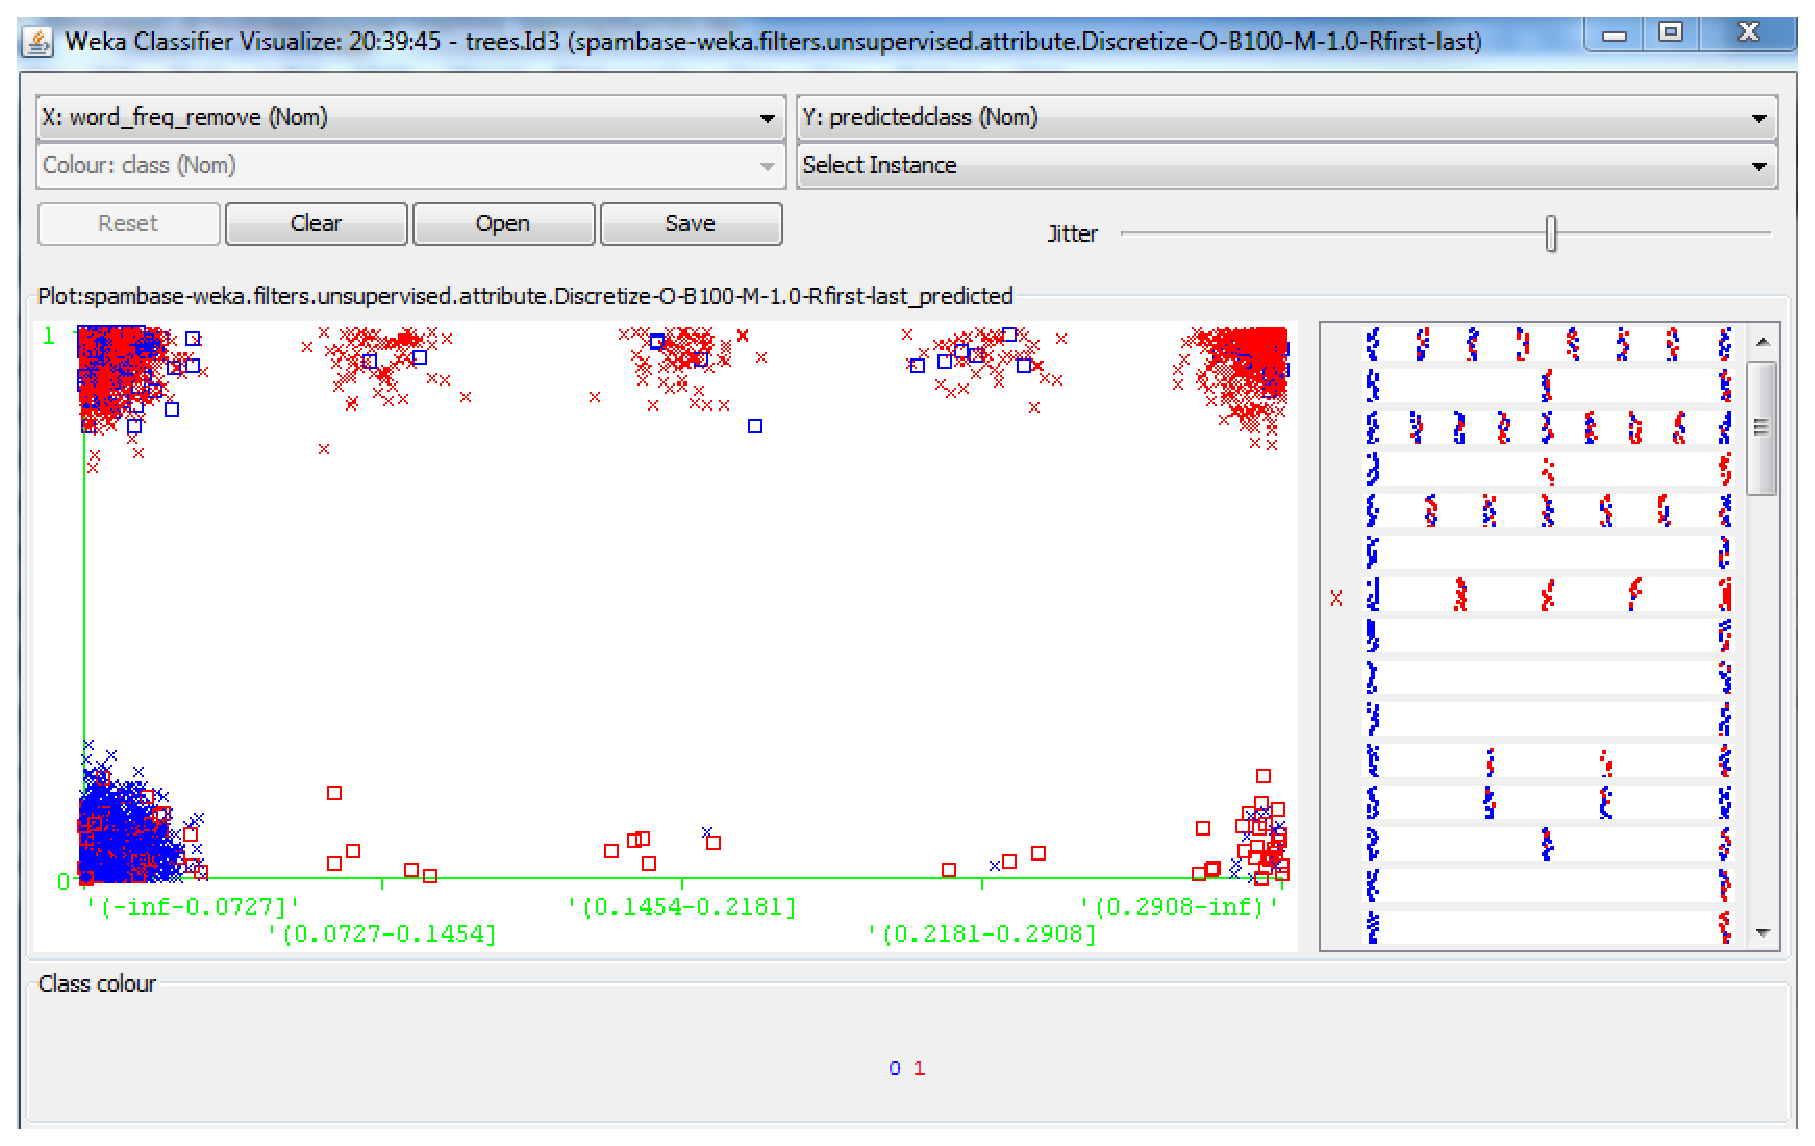
\includegraphics[width=0.8\textwidth]{eps/id3_unsupDiscrete_wordRemoveError}
	\caption{ID3 classifier error for the frequency of the word "remove".}
	\label{fig:id3_remove_error}
\end{figure}

\subsection{J48}
The J48 algorithm showed improvement over ID3 for all parameter combinations tested. The first parameter tested was the confidence factor. J48 was run with confidence values ranging from .25 to .85 with the minimum observations at each leaf set to 8. Figure \ref{fig:j48_confidence} shows that classification accuracy improves until .45 and then levels off at 92.35\%. This is due to the fact that J48 takes a pessimistic approach to deciding the error of each potential node. As you increase the confidence level, the model assumes that the error will be smaller and smaller. This improves accuracy until the model becomes overconfident.

\begin{figure}[here]
	\centering	
	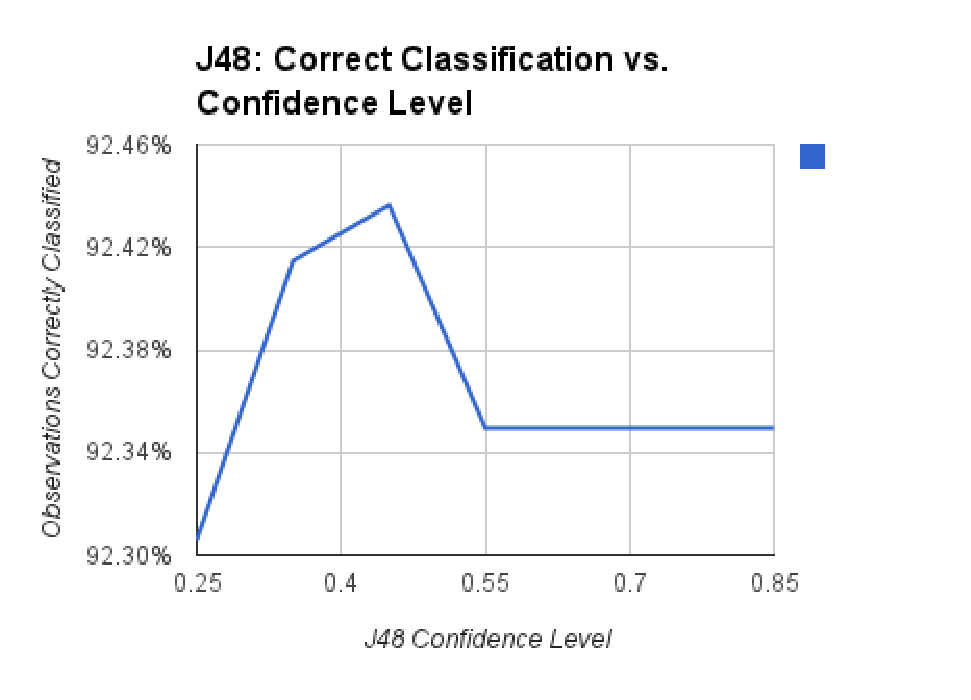
\includegraphics[width=0.5\textwidth]{eps/j48_confidence}
	\caption{J48 classification accuracy as confidence level increases.}
	\label{fig:j48_confidence}
\end{figure}

The J48 tree from the confidence tests had between 129 and 149 nodes. The minObjects parameter was then changed to observe its effect on the size of the tree. Figure \ref{fig:j48_min_objects} illustrates how the tree size decreases as minObjects increases. As you require more objects at each node, you are reducing the height of the tree. Correct classification starts at 92.98\% with minObject set to 2 and decreases to 90.28\% with a minimum of 32 objects per node.

\begin{figure}[here]
	\centering	
	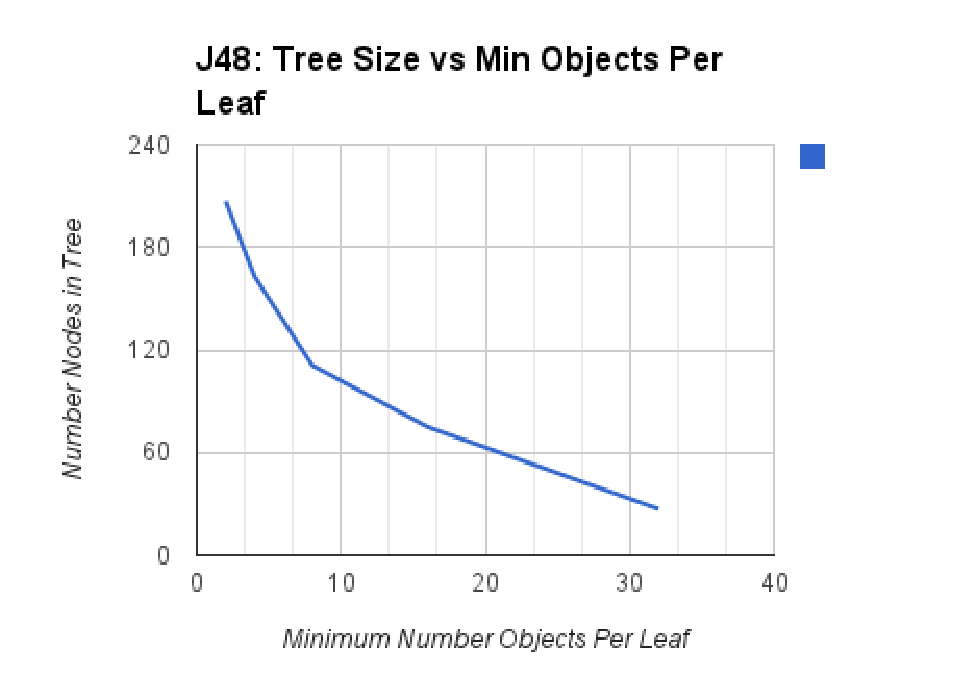
\includegraphics[width=0.5\textwidth]{eps/j48_min_objects}
	\caption{J48 tree size as minimum number of objects per leaf increases.}
	\label{fig:j48_min_objects}
\end{figure}

\section{Rule-Learning}
\subsection{Prism}
Prism generated a very complicated rule structure.
\subsection{JRip}
When JRip, with pruning, was run on the continuous dataset, it showed 92.39\% correctly classified instances using only 17 rules. After turning off pruning, JRip showed approximately the same accuracy at 92.13\%, but contained twice the rules at 35. Using 10-fold cross-validation, it seems that the un-pruned JRip was overfit to the training data. This may be why classification accuracy went up slightly when pruned.
\section{Exploration}
I have decided to used some of the theory regarding the construction of decision trees to my research on Content-Based Image Retrieval. There are many different image description algorithms that use histograms that describe frequencies of different image features. Color histograms would describe the number of pixels that are different colors, while shape histograms describe the presence of different shapes in different regions of an image. My goal for this project is to dynamically choose the most appropriate method based on a query image. 

Given a labeled set of training data containing different classes of images, e.g. buildings, cars, landscapes, histograms will be extracted for every image using several algorithms. For each bin in each histogram, the information gain will be calculated. The gain will be used to decide which algorithm to use for a query.

When a query image is submitted, then the histograms for all algorithms will be extracted from the image. The information gain for each algorithm will be calculated by summing the information gain of each detected attribute in the query image. The algorithm with the highest gain will be used to search the database. This will be the focus of my course project.
\section{Comparison of All Models}
Of the tree-based models, J48 showed the best classification accuracy, and the minObject feature along with pruning, allowed the tree size to be reduced greatly. However, the best algorithm tested was JRip due to the very high accuracy, while maintaining a relatively small set of rules at 17.
\section{References}

\bibliographystyle{plain}
\bibliography{references.bib}
\end{document}